\section{Run 2}

For the run $2$ of coursework $3$, the objective is to develop a set of linear classifiers for the classification task of our test set images. Before training the $15$ one vs all classifiers we need to represent our training, and later the test, images as bag of feature histograms, indeed we first need to define a vocabulary of visual words. A dictionary is represented by the centroids obtained from clustering using \textit{k-means}. The clusters are computed over the features collected across each image that makes the training set. The features that are going to be take in account in our model are $8\times 8$ patches, sampled at every $4$ pixels in $x$ and $y$ directions. The code for building a vocabulary is reported in \code{make\_vocabulary}, where, after import training images and splitting them between train set ($75\%$) and validation set ($25\%$), a dictionary is creating exploiting MATLAB's \textit{bagOfFeatures} function. It takes as input a training set, the size of vocabulary (which corresponds to the number of \textit{kmeans} clusters) and a custom features extraction function. This function, according to code in \code{myFeatureExtractor}, resizes input image to a $256\times 256$ picture in order to avoid problem with indexes in MATLAB and extract good features from image. It returns mean-centred, normalized patches representing the image.

At the end of this process, we ended up with \textit{k} ($500$ in default case) representative visual words (the centroid of each cluster). Once they have been computed, the following two steps are important for the final image representation before training classifiers. Firstly, we applied an "encoding" process that assigns at each $8\times 8$ patch within an image the closest word (nearest neighbour) in the dictionary. Secondly, each image is represented as a \textit{bag of words} (BOW) which is a histogram of the words, early computed, that together form the image. This type of representation is called a \textit{feature vector} representation of an image. By building a feature vector the system will be invariant to changes in the order of words, namely that it's invariant with respect to rotations, for example, of the image, which is a desirable property to exploit. This process is summarized in \code{get\_image\_bag} where the MATLAB's function \textit{encode} incorporates the two processes and produces a histogram that becomes a new and reduced representation of all the images inside training folder.

Finally, $15$ one-vs-all classifiers were trained. The classifiers are linear hence suitable for binary classification, but here we have a $15-way$ classification problem. Therefore, $15$ binary 1-vs-all support vector machines are trained in order to find a linear decision boundary. One vs all means that each classifier is trained to recognize object of a class with respect to all others. So , when training one of the classifiers, values from one class are taken and labelled as $1$ while other classes' values are labelled as $-1$, thus bringing back the problem to a binary classification problem for each classifiers combination. When making classification, input data is evaluated over all classifiers and final prediction corresponds to the classifier with highest predicted score. As reported in \code{run2}, classifiers are trained using \textit{vl\_svmtrain} function provided by VL-FEAT [1].
This function receives, among training data and labels, an important tunable parameter \textit{lambda}, that controls the learning rate for each SVM. In this code the prediction accuracy is evaluated over validation set (for different configurations and values for \textit{lambda}) and all images in "testing" folder are classified.

\begin{figure}[!htbp] 
	\centering
	{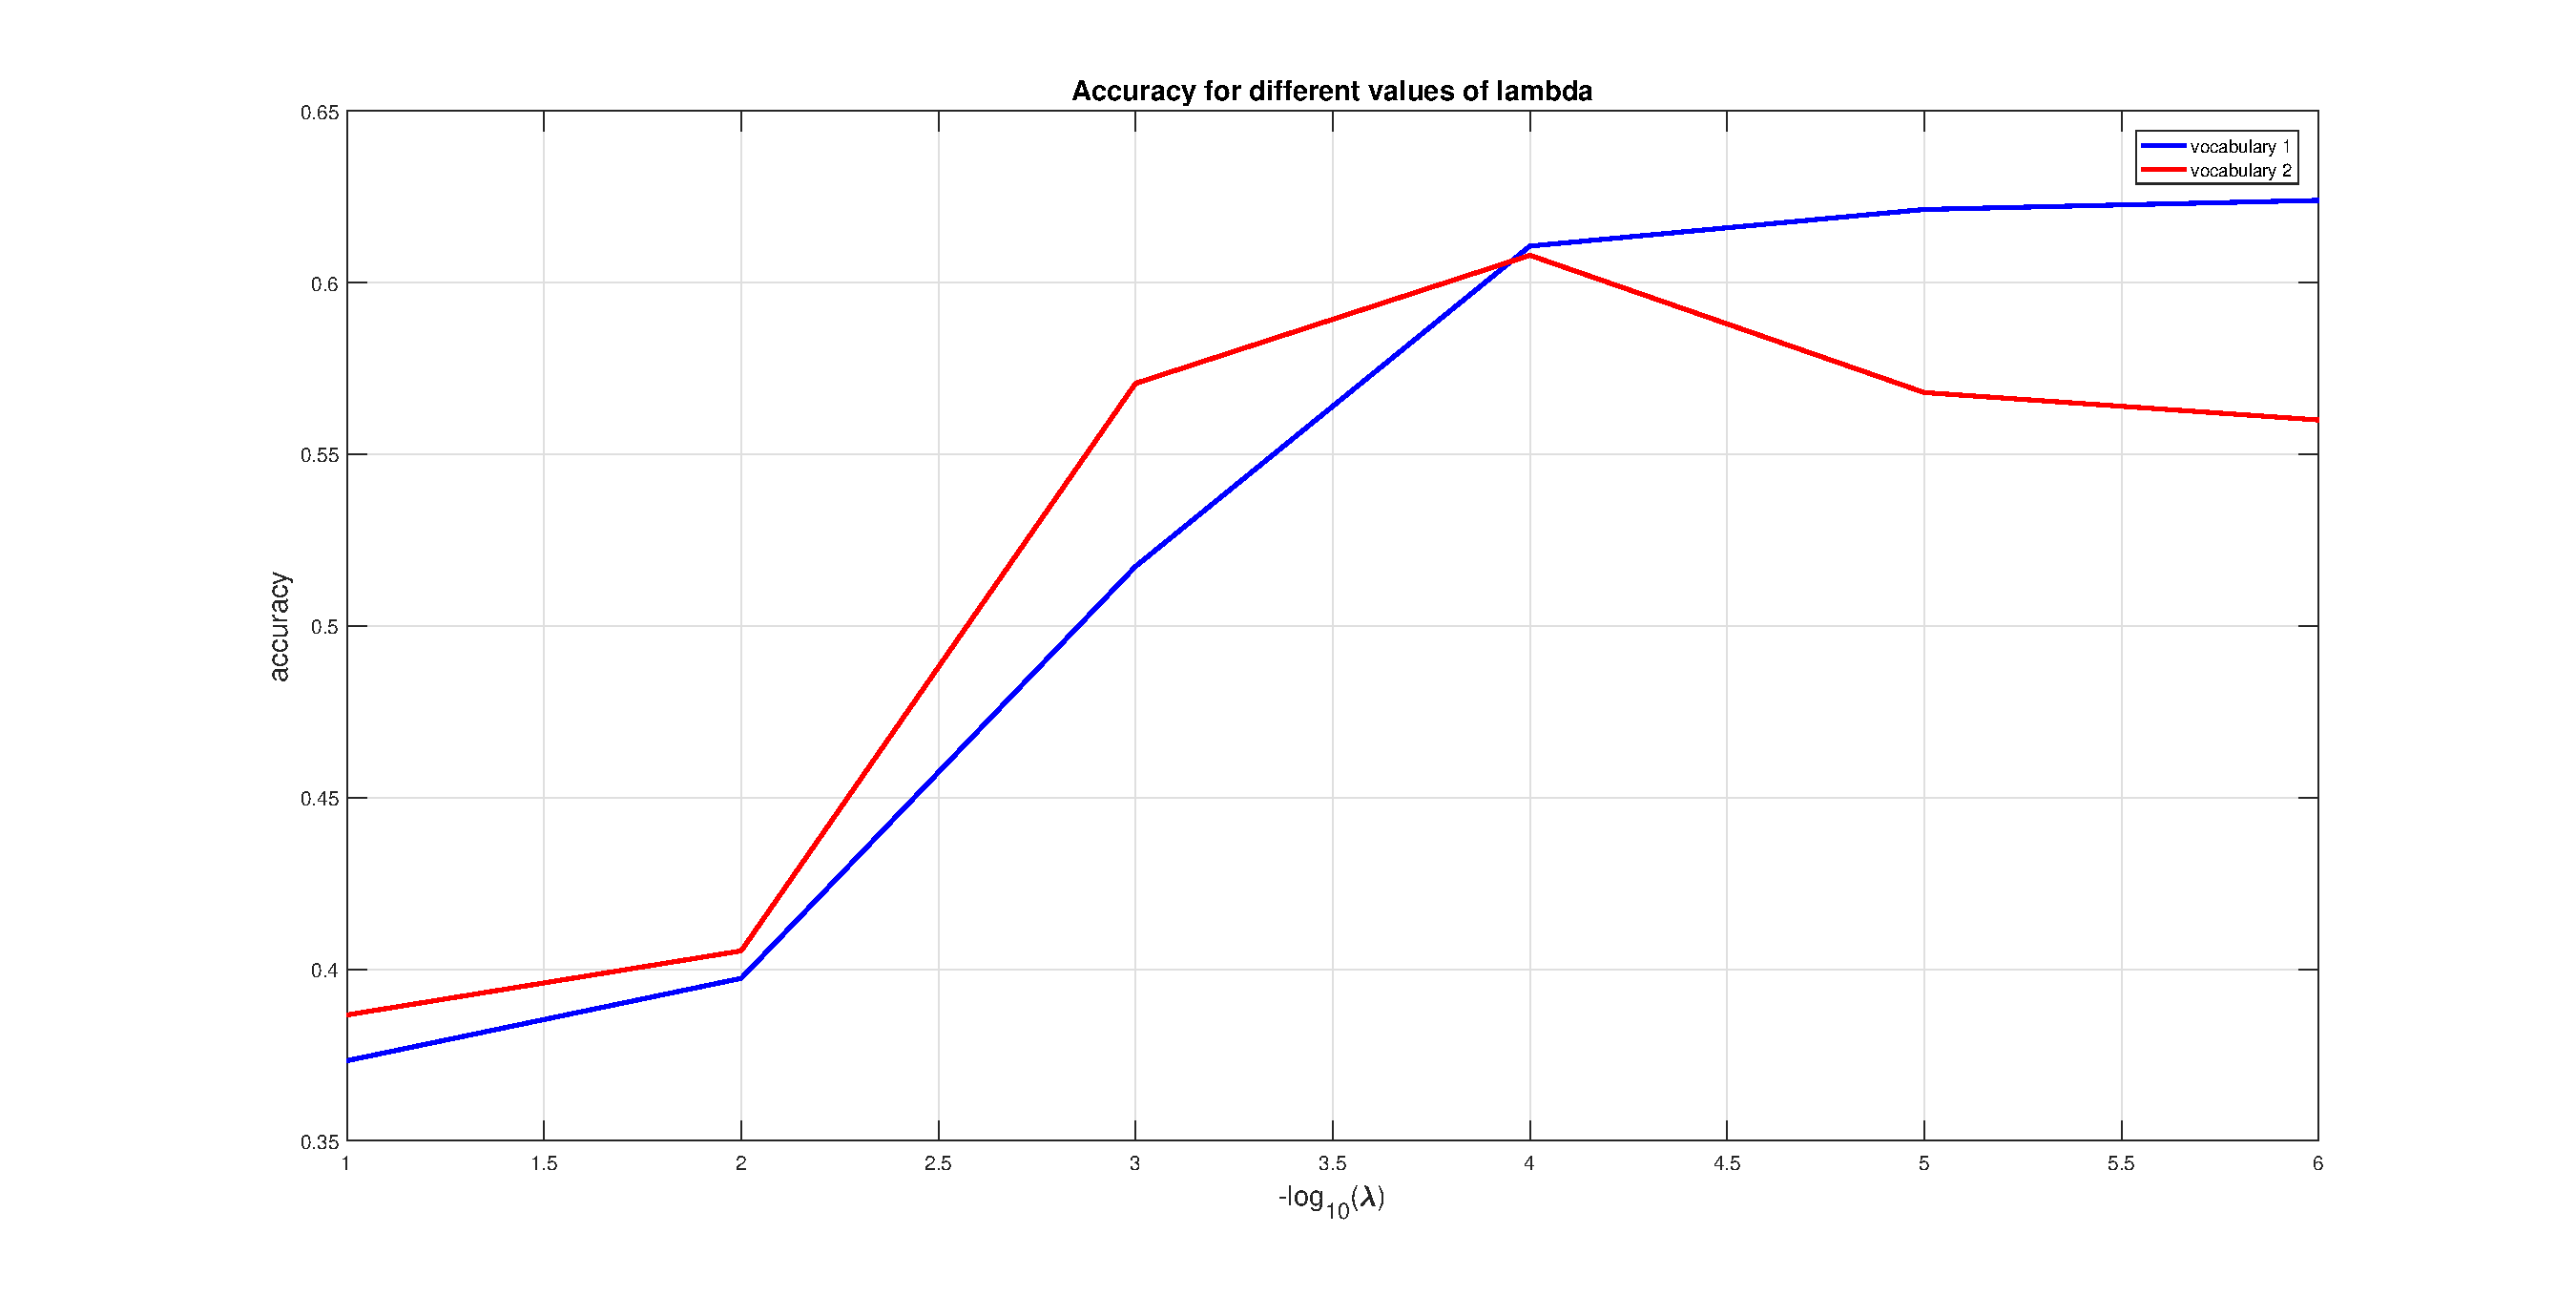
\includegraphics[width=.5\linewidth]{./run2.eps}}
	\caption{Accuracy comparison for different lambda values and dictionaries.}
	\label{fig:run2}
\end{figure}

In Fig. \ref{fig:run2}, it's reported an accuracy comparison considering two dictionaries: \textit{vocabulary 1} has been obtained with default patch size and has $500$ words, while \textit{vocabulary 2} consists of $4\times 4$ patches 